

%🍁% \chapter{Iteration  |  迭代}
\chapter{迭代}

%🍁% This chapter is about iteration, which is the ability to run
%🍁% a block of statements repeatedly.  We saw a kind of iteration,
%🍁% using recursion, in Section~\ref{recursion}.
%🍁% We saw another kind, using a {\tt for} loop,
%🍁% in Section~\ref{repetition}.  In this chapter we'll see yet another
%🍁% kind, using a {\tt while} statement.
%🍁% But first I want to say a little more about variable assignment.

本章介绍迭代,即重复运行某个代码块的能力。我们已经在~\ref{recursion} 节接触了一种利用递归进行迭代的方式;在~\ref{repetition} 节中,接触了另一种利用 \li{for} 循环进行迭代的方式。 在本章中,我们将讨论另外一种利用 \li{while} 语句实现迭代的方式。
不过,首先我想再多谈谈有关变量赋值的问题。

%🍁%  \section{Reassignment  |  重新赋值}
\section{重新赋值}
\index{assignment}  \index{statement!assignment}  \index{reassignment}
\index{赋值}  \index{语句!赋值}  \index{重新赋值}

%🍁% As you may have discovered, it is legal to make more than one
%🍁% assignment to the same variable.  A new assignment makes an existing
%🍁% variable refer to a new value (and stop referring to the old value).

可能你已发现对同一变量进行多次赋值是合法的。 新的赋值会使得已有的变量指向
新的值(同时不再指向旧的值)。

\begin{lstlisting}
>>> x = 5
>>> x
5
>>> x = 7
>>> x
7
\end{lstlisting}

%
%🍁% The first time we display
%🍁% {\tt x}, its value is 5; the second time, its
%🍁% value is 7.

第一次打印 \li{x} 时, 它的值为 \li{5};第二次打印时,它的值是 \li{7}。

%🍁% Figure~\ref{fig.assign2} shows what {\bf reassignment} looks
%🍁% like in a state diagram.
%🍁% \index{state diagram} \index{diagram!state}

图~\ref{fig.assign2} 展示了 {\bf 重新赋值} 在状态图中看起来是什么样子。
\index{state diagram} \index{diagram!state}

%🍁% At this point I want to address a common source of confusion.
%🍁% Because Python uses the equal sign ({\tt =}) for assignment, it is
%🍁% tempting to interpret a statement like {\tt a = b} as a mathematical
%🍁% proposition of equality; that is, the claim that {\tt a} and
%🍁% {\tt b} are equal.  But this interpretation is wrong.
%🍁% \index{equality and assignment}

这里我想探讨一个常见的疑惑点。由于 Python 用等号 (\li{=}) 来赋值,所以很容易将 \li{a = b} 这样的语句理解为数学上的相等命题;即 \li{a} 和 \li{b} 相等。但是这种理解是错误的。

%🍁% First, equality is a symmetric relationship and assignment is not.  For
%🍁% example, in mathematics, if $a=7$ then $7=a$.  But in Python, the
%🍁% statement {\tt a = 7} is legal and {\tt 7 = a} is not.

首先,相等是一种对称关系,赋值不是。例如,在数学上,如果 $a = 7$,
则 $7 = a$。 但是在 Python 中,语句 \li{a = 7} 是合法的, \li{7 = a} 则不合法。

%🍁% Also, in mathematics, a proposition of equality is either true or
%🍁% false for all time.  If $a=b$ now, then $a$ will always equal $b$.
%🍁% In Python, an assignment statement can make two variables equal, but
%🍁% they don't have to stay that way:

此外,数学中,相等命题不是对的就是错的。 如果 $a = b$,那么 $a$
则是永远与 $b$ 相等。在 Python 中,赋值语句可以使得两个变量相等,
但是这两个变量不一定必须保持这个状态:


\begin{lstlisting}
>>> a = 5
>>> b = a    # a and b are now equal
>>> a = 3    # a and b are no longer equal
>>> b
5
\end{lstlisting}

%
%🍁% The third line changes the value of {\tt a} but does not change the
%🍁% value of {\tt b}, so they are no longer equal.

第三行改变了 \li{a} 的值,但是没有改变 \li{b} 的值,所以它们不再相等了。

%🍁% Reassigning variables is often useful, but you should use it
%🍁% with caution.  If the values of variables change frequently, it can
%🍁% make the code difficult to read and debug.

给变量重新赋值非常有用,但是需要小心使用。 对变量频繁重新赋值会使代码难于阅读,
不易调试。

\begin{figure}
\centerline
{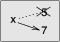
\includegraphics[scale=0.99]{../source/figs/assign2.pdf}}
% \caption {State diagram.}
\caption {重新赋值的状态图。}
\label{fig.assign2}
\end{figure}


%🍁% \section{Updating variables  |  更新变量}
\section{更新变量}
\label{update}

\index{update}  \index{variable!updating}
\index{更新}  \index{变量!更新}

%🍁% A common kind of reassignment is an {\bf update},
%🍁% where the new value of the variable depends on the old.

重新赋值的一个常见方式是 {\em 更新} (update) , 更新操作中变量的新值会取决于旧值。


\begin{lstlisting}
>>> x = x + 1
\end{lstlisting}

%
%🍁% This means ``get the current value of {\tt x}, add one, and then
%🍁% update {\tt x} with the new value.''

这个语句的意思是,``获得 \li{x} 的当前值并与 \li{1} 做加法求和,然后将 \li{x} 的值更新为所求的和。''

%🍁% If you try to update a variable that doesn't exist, you get an
%🍁% error, because Python evaluates the right side before it assigns
%🍁% a value to {\tt x}:

如果试图去更新一个不存在的变量,则会返回一个错误。 这是因为 Python 是先求
式子右边的值,然后再把所求的值赋给 \li{x}:

\begin{lstlisting}
>>> x = x + 1
NameError: name 'x' is not defined
\end{lstlisting}

%
%🍁% Before you can update a variable, you have to {\bf initialize}
%🍁% it, usually with a simple assignment:
%🍁% \index{initialization (before update)}

在更新变量之前,你得先 {\em 初始化} (initialize) 它,通常是通过一个简单的赋值实现:
\index{initialization (before update)}
\index{初始化}

\begin{lstlisting}
>>> x = 0
>>> x = x + 1
\end{lstlisting}

%
%🍁% Updating a variable by adding 1 is called an {\bf increment};
%🍁% subtracting 1 is called a {\bf decrement}.
%🍁% \index{increment}  \index{decrement}

通过加 \li{1} 来更新变量叫做 {\em 递增} (increment); 减 \li{1} 叫做 {\em 递减} (decrement)。
\index{increment}  \index{decrement}
\index{递增}  \index{递减}


%🍁% \section{The {\tt while} statement  |  {\tt while} 语句}
\section{{\tt while} 语句}

\index{statement!while}  \index{while loop}
\index{loop!while}  \index{iteration}


%🍁% Computers are often used to automate repetitive tasks.  Repeating
%🍁% identical or similar tasks without making errors is something that
%🍁% computers do well and people do poorly.  In a computer program,
%🍁% repetition is also called {\bf iteration}.

计算机经常被用来自动处理重复性的任务。
计算机很擅长无纰漏地重复相同或者相似的任务, 而人类在这方面做的不好。
在计算机程序中, 重复也被称为 {\em 迭代} (iteration)。

%🍁% We have already seen two functions, {\tt countdown} and
%🍁% \verb"print_n", that iterate using recursion.  Because iteration is so
%🍁% common, Python provides language features to make it easier.
%🍁% One is the {\tt for} statement we saw in Section~\ref{repetition}.
%🍁% We'll get back to that later.

我们已经见过两个利用递归来迭代的函数: \li{countdown} 和 \li{print_n} 。 由于迭代的使用非常普遍, 所以 Python 提供了使其更容易实现的语言特性。 其中之一就是我们在 \ref{repetition}~节 看到的 \li{for} 语句。 后面我们还会继续介绍。

% add hyperref of 后面 here

%🍁% Another is the {\tt while} statement.  Here is a version of {\tt
%🍁% countdown} that uses a {\tt while} statement:

另外一个用于迭代的语句是 \li{while} 。 下面是使用 \li{while} 语句实现的 \li{countdown}:

\begin{lstlisting}
def countdown(n):
    while n > 0:
        print(n)
        n = n - 1
    print('Blastoff!')
\end{lstlisting}

%
%🍁% You can almost read the {\tt while} statement as if it were English.
%🍁% It means, ``While {\tt n} is greater than 0,
%🍁% display the value of {\tt n} and then decrement
%🍁% {\tt n}.  When you get to 0, display the word {\tt Blastoff!}''
\index{flow of execution}

你可以像读英语句子一样来读 \li{while} 语句。 它的意思是:``只要 \li{n} 的值大于 \li{0}, 则打印出 \li{n} 的值,然后让 \li{n} 减 \li{1}。 当 \li{n} 递减至 \li{0} 时,打印单词 \li{Blastoff}!''。

%🍁% More formally, here is the flow of execution for a {\tt while} statement:

更正式地来说,\li{while} 语句的执行流程如下:

%🍁% \begin{enumerate}
%🍁%
%🍁% \item Determine whether the condition is true or false.
%🍁%
%🍁% \item If false, exit the {\tt while} statement
%🍁% and continue execution at the next statement.
%🍁%
%🍁% \item If the condition is true, run the
%🍁% body and then go back to step 1.
%🍁%
%🍁% \end{enumerate}

\begin{enumerate}

\item 首先判断条件为 {\bf 真} 还是为 {\bf 假}。

\item 如果为假,退出 \li{while} 语句,然后执行接下来的语句;

\item 如果条件为真,则运行 \li{while} 语句 {\em 循环主体},运行完再返回第一步;

\end{enumerate}

%🍁% This type of flow is called a loop because the third step
%🍁% loops back around to the top.
\index{condition}  \index{loop}  \index{body}

这种形式的流程叫做 {\em 循环} (loop), 因为第三步后又循环回到了第一步。
\index{条件}  \index{循环}  \index{循环体}

%🍁% The body of the loop should change the value of one or more variables
%🍁% so that the condition becomes false eventually and the loop
%🍁% terminates.  Otherwise the loop will repeat forever, which is called
%🍁% an {\bf infinite loop}.  An endless source of amusement for computer
%🍁% scientists is the observation that the directions on shampoo,
%🍁% ``Lather, rinse, repeat'', are an infinite loop.
\index{infinite loop}  \index{loop!infinite}

循环主体应该改变一个或多个变量的值,这样的话才能让条件判断最终变为假,
从而终止循环。 否则,循环将会永远重复下去,这被称为 {\em 无限循环} (infinite loop)。 在计算机科学家看来,洗发水的使用说明 —— ``抹洗发水,
清洗掉,重复'' 便是个无限循环,这总是会让他们觉得好笑。
\index{无限循环}  \index{循环!无限}

%🍁% In the case of {\tt countdown}, we can prove that the loop
%🍁% terminates: if {\tt n} is zero or negative, the loop never runs.
%🍁% Otherwise, {\tt n} gets smaller each time through the
%🍁% loop, so eventually we have to get to 0.

对于 \li{countdown} 来说,我们可以证明循环是一定会终止的:当 n 是 0 或者负数,该循环就不会执行;不然 n 通过每次循环之后慢慢减小,最终也是会变成 0 的。

%🍁% For some other loops, it is not so easy to tell.  For example:

有些其他循环,可能就没那么好理解了。例如:

\begin{lstlisting}
def sequence(n):
    while n != 1:
        print(n)
        if n % 2 == 0:        # n is even
            n = n / 2
        else:                 # n is odd
            n = n*3 + 1
\end{lstlisting}

%
%🍁% The condition for this loop is {\tt n != 1}, so the loop will continue
%🍁% until {\tt n} is {\tt 1}, which makes the condition false.

循环的条件是 \li{n != 1},所以循环会一直执行到 \li{n} 等于 \li{1},条件判断为假时循环才终止。

%🍁% Each time through the loop, the program outputs the value of {\tt n}
%🍁% and then checks whether it is even or odd.  If it is even, {\tt n} is
%🍁% divided by 2.  If it is odd, the value of {\tt n} is replaced with
%🍁% {\tt n*3 + 1}. For example, if the argument passed to {\tt sequence}
%🍁% is 3, the resulting values of {\tt n} are 3, 10, 5, 16, 8, 4, 2, 1.

每次循环,该程序打印出 \li{n} 的值,然后检查它是偶数还是奇数。如果它是偶数,
那么 \li{n} 可以被2整除;如果是奇数,则它的值被替换为 \li {n*3 + 1}。 例如,如果传递给 \li{sequence} 的实参为3, 那么打印出的结果将会是:\li{3}、 \li{10}、 \li{5}、 \li{16}、 \li{8}、 \li{4}、 \li{2}、 \li{1}。

%🍁% Since {\tt n} sometimes increases and sometimes decreases, there is no
%🍁% obvious proof that {\tt n} will ever reach 1, or that the program
%🍁% terminates.  For some particular values of {\tt n}, we can prove
%🍁% termination.  For example, if the starting value is a power of two,
%🍁% {\tt n} will be even every time through the loop
%🍁% until it reaches 1. The previous example ends with such a sequence,
%🍁% starting with 16.
%🍁% \index{Collatz conjecture}

由于 \li{n} 的值时增时减,所以不能轻易保证 \li{n} 会最终变成 \li{1}, 或者说这个程序能够终止。 对于某些特殊的 \li{n} 的值,可以很好地证明它是可以终止的。 例如, 当 \li{n} 的初始值是 \li{2} 的倍数时,则每次循环后 \li{n} 一直为偶数, 直到最终变为 \li{1}。 上一个示例中,程序就打印了类似的序列, 从 \li{16} 开始全部为偶数。
\index{Collatz conjecture}

%🍁% The hard question is whether we can prove that this program terminates
%🍁% for {\em all} positive values of {\tt n}.  So far, no one has
%🍁% been able to prove it {\em or} disprove it!  (See
%🍁%   \url{http://en.wikipedia.org/wiki/Collatz_conjecture}.)

难点在于是否能证明程序对于 {\bf 所有} 的正整数 \li{n} 都会终止。 目前为止,
还没有人证明 {\bf 或者} 证伪该命题\footnote{见:\href{http://en.wikipedia.org/wiki/Collatz_conjecture}{考拉兹猜想}}。
\index{考拉兹猜想}  \index{维基百科}

%🍁% As an exercise, rewrite the function \verb"print_n" from
%🍁% Section~\ref{recursion} using iteration instead of recursion.

我们做个练习,利用迭代而非递归,重写之前~\ref{recursion} 节中的 \li{print_n} 函数。

%🍁% \section{{\tt break} }
\section{{\tt break} }
\index{break statement}  \index{statement!break}

%🍁% Sometimes you don't know it's time to end a loop until you get half
%🍁% way through the body.  In that case you can use the {\tt break}
%🍁% statement to jump out of the loop.

有些时候循环执行到一半你才知道循环该结束了。这种情况下,你可以使用 \li{break} 语句来跳出循环。

%🍁% For example, suppose you want to take input from the user until they
%🍁% type {\tt done}.  You could write:

例如,假设你想从用户那里获取输入,直到用户键入 \li{'done'}。 你可以这么写:

\begin{lstlisting}
while True:
    line = input('> ')
    if line == 'done':
        break
    print(line)

print('Done!')
\end{lstlisting}

%
%🍁% The loop condition is {\tt True}, which is always true, so the
%🍁% loop runs until it hits the break statement.

循环条件是 \li{True},其总是为真,所以该循环会一直执行直到碰到 \li{break}。

%🍁% Each time through, it prompts the user with an angle bracket.
%🍁% If the user types {\tt done}, the {\tt break} statement exits
%🍁% the loop.  Otherwise the program echoes whatever the user types
%🍁% and goes back to the top of the loop.  Here's a sample run:

每次循环时,程序都会给出一个尖括号 (\li{>}) 提示。 如果用户输入 \li{'done'},执行 \li{break} 语句跳出循环。 否则, 程序就会一直打印出用户所输入的内容并且跳到循环开始, 0以下是一个运行示例:


\begin{lstlisting}
> not done
not done
> done
Done!
\end{lstlisting}

%
%🍁% This way of writing {\tt while} loops is common because you
%🍁% can check the condition anywhere in the loop (not just at the
%🍁% top) and you can express the stop condition affirmatively
%🍁% (``stop when this happens'') rather than negatively (``keep going
%🍁% until that happens'').

\li{while} 循环的这种写法很常见, 因为你可以在循环的任何地方判断条件
(而不只是在循环开始), 而且你可以积极地表达终止条件(``当出现这个情况是终止''), 而不是消极地表示 (``继续运行直到出现这个情况'')。


%🍁% \section{Square roots  |  平方根}
\section{平方根}
\label{squareroot}
\index{square root}  \index{平方根}

%🍁% Loops are often used in programs that compute
%🍁% numerical results by starting with an approximate answer and
%🍁% iteratively improving it.
\index{Newton's method}

循环常用于计算数值的程序中, 这类程序一般从一个大概的值开始, 然后迭代式地进行改进。
\index{牛顿法}

%🍁% For example, one way of computing square roots is Newton's method.
%🍁% Suppose that you want to know the square root of $a$.  If you start
%🍁% with almost any estimate, $x$, you can compute a better
%🍁% estimate with the following formula:

例如,牛顿法 (Newton's method) 是计算平方根的一种方法。 假设你想求 $a$ 的平方根。 如果你从任意一个估算值 $x$ 开始, 则可以利用下面的公式计算出更为较为精确的估算值:

\[ y = \frac{x + a/x}{2} \]

%
%🍁% For example, if $a$ is 4 and $x$ is 3:

例如,假定 $a$ 是 4,$x$ 是 3:

\begin{lstlisting}
>>> a = 4
>>> x = 3
>>> y = (x + a/x) / 2
>>> y
2.16666666667
\end{lstlisting}

%
%🍁% The result is closer to the correct answer ($\sqrt{4} = 2$).  If we
%🍁% repeat the process with the new estimate, it gets even closer:

可以看到, 结果与真实值 ( $\sqrt{4} = 2$ ) 已经很接近了, 如果我们用这个值
再重新运算一遍, 它将得到更为接近的值。


\begin{lstlisting}
>>> x = y
>>> y = (x + a/x) / 2
>>> y
2.00641025641
\end{lstlisting}

%
%🍁% After a few more updates, the estimate is almost exact:
%🍁% \index{update}

再通过多几次的运算,这个估算可以说已经是很精确了。
\index{update}

\begin{lstlisting}
>>> x = y
>>> y = (x + a/x) / 2
>>> y
2.00001024003
>>> x = y
>>> y = (x + a/x) / 2
>>> y
2.00000000003
\end{lstlisting}

%
%🍁% In general we don't know ahead of time how many steps it takes
%🍁% to get to the right answer, but we know when we get there
%🍁% because the estimate
%🍁% stops changing:

一般来说, 我们事先不知道要多少步才能得到正确答案, 但是我们知道当估算值不再变动时, 我们就获得了正确的答案。

\begin{lstlisting}
>>> x = y
>>> y = (x + a/x) / 2
>>> y
2.0
>>> x = y
>>> y = (x + a/x) / 2
>>> y
2.0
\end{lstlisting}

%
%🍁% When {\tt y == x}, we can stop.  Here is a loop that starts
%🍁% with an initial estimate, {\tt x}, and improves it until it
%🍁% stops changing:

当 \li{y == x} 时,我们可以停止计算了。下面这个循环就是利用一个初始估值 \li{x},
循序渐进地计算,直到估值不再变化。

\begin{lstlisting}
while True:
    print(x)
    y = (x + a/x) / 2
    if y == x:
        break
    x = y
\end{lstlisting}

%
%🍁% For most values of {\tt a} this works fine, but in general it is
%🍁% dangerous to test {\tt float} equality.
%🍁% Floating-point values are only approximately right:
%🍁% most rational numbers, like $1/3$, and irrational numbers, like
%🍁% $\sqrt{2}$, can't be represented exactly with a {\tt float}.
%🍁% \index{floating-point}  \index{epsilon}

对于大部分 \li{a} 的值,这个程序运行正常,不过一般来说,检查两个浮点数是否相等比较危险。浮点数只能大约表示:大多数有理数,如 $1/3$,以及无理数,
如 : $\sqrt{2}$,是不能用浮点数 ( \li{float} ) 来精确表示的。
\index{floating-point}  \index{epsilon}

%🍁% Rather than checking whether {\tt x} and {\tt y} are exactly equal, it
%🍁% is safer to use the built-in function {\tt abs} to compute the
%🍁% absolute value, or magnitude, of the difference between them:

与其检查 \li{x} 和 \li{y} 的值是否完全相等,使用内置函数 \li{abs} 来计算二者之差的绝对值或数量级更为安全:

\begin{lstlisting}
    if abs(y-x) < epsilon:
        break
\end{lstlisting}

%
%🍁% Where \verb"epsilon" has a value like {\tt 0.0000001} that
%🍁% determines how close is close enough.

这里,变量 \li{epsilon} 是一个决定其精确度的值,如 \li{0.0000001}。

%🍁% \section{Algorithms  |  算法}
\section{算法}
\index{algorithm}  \index{算法}

%🍁% Newton's method is an example of an {\bf algorithm}: it is a
%🍁% mechanical process for solving a category of problems (in this
%🍁% case, computing square roots).

牛顿法就是一个 {\em 算法} (Algorithm) 示例: 它是解决一类问题的计算机制 (本例中是计算平方根)。

%🍁% To understand what an algorithm is, it might help to start with
%🍁% something that is not an algorithm.  When you learned to multiply
%🍁% single-digit numbers, you probably memorized the multiplication table.
%🍁% In effect, you memorized 100 specific solutions.  That kind of
%🍁% knowledge is not algorithmic.

为了理解算法是什么,先了解什么不是算法或许有点帮助。 你在学习一位数乘法时,
可能背出了乘法表。 实际上,你只是记住了 100 个确切的答案。 这种知识并{\bf 不是}算法性的。

%🍁% But if you were ``lazy'', you might have learned a few
%🍁% tricks.  For example, to find the product of $n$ and 9, you can
%🍁% write $n-1$ as the first digit and $10-n$ as the second
%🍁% digit.  This trick is a general solution for multiplying any
%🍁% single-digit number by 9.  That's an algorithm!
%🍁% \index{addition with carrying}  \index{carrying, addition with}
%🍁% \index{subtraction!with borrowing}  \index{borrowing, subtraction with}

不过, 如果你想找 ``懒人方法'', 你可能就会找到一些诀窍。 比如为了计算 $n$
和 $9$ 的乘积,你可以把 $n-1$ 作为乘积的第一位数,再把 $10-n$
作为第二位数,从而得到它们的乘积。 这个诀窍是将任意个位数
与 $9$ 相乘的普遍解法。 这就{\bf 是}一种算法。
\index{addition with carrying}  \index{carrying, addition with}
\index{subtraction!with borrowing}  \index{borrowing, subtraction with}

%🍁% Similarly, the techniques you learned for addition with carrying,
%🍁% subtraction with borrowing, and long division are all algorithms.  One
%🍁% of the characteristics of algorithms is that they do not require any
%🍁% intelligence to carry out.  They are mechanical processes where
%🍁% each step follows from the last according to a simple set of rules.

类似地,你所学过的进位加法、借位减法、以及长除法都是算法。算法的特点之一
就是不需要过多的脑力计算。算法是一个机械的过程,每一步都是依
据一组简单的规则跟着上一步来执行的。

%🍁% Executing algorithms is boring, but designing them is interesting,
%🍁% intellectually challenging, and a central part of computer science.

执行算法的过程是很乏味的,但是设计算法就比较有趣了,不但是智
力上的挑战,更是计算机科学的核心。

%🍁% Some of the things that people do naturally, without difficulty or
%🍁% conscious thought, are the hardest to express algorithmically.
%🍁% Understanding natural language is a good example.  We all do it, but
%🍁% so far no one has been able to explain {\em how} we do it, at least
%🍁% not in the form of an algorithm.

一些人们自然而然无需下意识做到的事情,往往是难于用算法表达。 理解自然语言就是这样的。 我们每个人都听得懂自然语言, 但是目前还没有人能够解释我们是 {\bf 怎么} 做到的, 至少无法以算法的形式解释。

%🍁% \section{Debugging  |  调试}
\section{调试}
\label{bisectbug}

%🍁% As you start writing bigger programs, you might find yourself
%🍁% spending more time debugging.  More code means more chances to
%🍁% make an error and more places for bugs to hide.
%🍁% \index{debugging!by bisection}  \index{bisection, debugging by}

当你开始写更为复杂的程序时,你会发现大部分时间都花费在调试上。 更多的
代码意味着更高的出错概率,并且会有更多隐藏 bug 的地方。
\index{debugging!by bisection}  \index{bisection, debugging by}

%🍁% One way to cut your debugging time is ``debugging by bisection''.
%🍁% For example, if there are 100 lines in your program and you
%🍁% check them one at a time, it would take 100 steps.

减少调试时间的一个方法就是“对分调试”。例如,如果程序有100行,你一次检查一行,就需要100步。

%🍁% Instead, try to break the problem in half.  Look at the middle
%🍁% of the program, or near it, for an intermediate value you
%🍁% can check.  Add a {\tt print} statement (or something else
%🍁% that has a verifiable effect) and run the program.

相反, 试着将问题拆为两半。 在代码中间部分或者附近的地方, 寻找一个可以检查的中间值。 加上一行 \li{print} 语句 (或是其他具有可验证效果的代码), 然后运行程序。

%🍁% If the mid-point check is incorrect, there must be a problem in the
%🍁% first half of the program.  If it is correct, the problem is
%🍁% in the second half.

如果中间点检查出错了, 那么就说明程序的前半部分存在问题。 如果没问题, 则说明是后半部分出错了。

%🍁% Every time you perform a check like this, you halve the number of
%🍁% lines you have to search.  After six steps (which is fewer than 100),
%🍁% you would be down to one or two lines of code, at least in theory.

每次你都这样检查, 就可以将需要搜索的代码行数减少一半。 经过6步之后 (这比100小多了), 你将会找到那或者两行出错的代码, 至少理论上是这样。

%🍁% In practice it is not always clear what
%🍁% the ``middle of the program'' is and not always possible to
%🍁% check it.  It doesn't make sense to count lines and find the
%🍁% exact midpoint.  Instead, think about places
%🍁% in the program where there might be errors and places where it
%🍁% is easy to put a check.  Then choose a spot where you
%🍁% think the chances are about the same that the bug is before
%🍁% or after the check.

在实践中, 可能并不能很好的确定程序的 ``中间部分'' 是什么, 也有可能并不是那么好检查。
计算行数并且取其中间行是没有意义的。 相反, 多考虑下程序中哪些地方比较容易出问题, 或者哪些地方比较容易进行检查。 然后选定一个检查点, 在这个断点前后出现bug的概念差不多。

%🍁% \section{Glossary  |  术语表}
\section{术语表}

\begin{description}

%🍁% \item[reassignment:] Assigning a new value to a variable that
%🍁% already exists.
%🍁% \index{reassignment}

\item[重新赋值 (reassignment):] 给已经存在的变量赋一个新的值。
\index{reassignment}

%🍁% \item[update:] An assignment where the new value of the variable
%🍁% depends on the old.
%🍁% \index{update}

\item[更新 (update):] 变量的新值取决于旧值的一种赋值方法。
\index{update}

%🍁% \item[initialization:] An assignment that gives an initial value to
%🍁% a variable that will be updated.
%🍁% \index{initialization!variable}

\item[初始化 (initialize):] 给后面将要更新的变量一个初始值的一种赋值方法。
\index{initialization!variable}

%🍁% \item[increment:] An update that increases the value of a variable
%🍁% (often by one).
%🍁% \index{increment}

\item[递增 (increment):] 通过增加变量的值的方式更新变量 (通常是加 1)。
\index{increment}

%🍁% \item[decrement:] An update that decreases the value of a variable.
%🍁% \index{decrement}

\item[递减 (decrement):] 通过减少变量的值的方式来更新变量。
\index{decrement}

%🍁% \item[iteration:] Repeated execution of a set of statements using
%🍁% either a recursive function call or a loop.
%🍁% \index{iteration}

\item[迭代 (iteration):] 利用递归或者循环的方式来重复执行代一组语句的过程。
\index{iteration}

%🍁% \item[infinite loop:] A loop in which the terminating condition is
%🍁% never satisfied.
%🍁% \index{infinite loop}

\item[无限循环 (infinite loop):] 无法满足终止条件的循环。
\index{infinite loop}

%🍁% \item[algorithm:]  A general process for solving a category of
%🍁% problems.
%🍁% \index{algorithm}

\item[算法 (algorithm):] 解决一类问题的通用过程。
\index{algorithm}

\end{description}

%🍁% \section{Exercises  |  练习}
\section{练习}

\begin{exercise}
\index{algorithm!square root}

%🍁% Copy the loop from Section~\ref{squareroot}
%🍁% and encapsulate it in a function called
%🍁% \verb"mysqrt" that takes {\tt a} as a parameter, chooses a
%🍁% reasonable value of {\tt x}, and returns an estimate of the square
%🍁% root of {\tt a}.  \index{encapsulation}

复制{\em \ref{squareroot}}~小节中的循环, 将其封装进一个叫 {\em \li{mysqrt}} 的函数中。 这个函数接受 {\em \li{a}} 作为形参,选择一个合适的 {\em \li{x}} 值,并返回 {\em \li{a}} 的平方根估算值。

%🍁% To test it, write a function named \verb"test_square_root"
%🍁% that prints a table like this:

为测试上面的函数,编写一个名为 {\em \li{test_squre_root}} 的函数,打印出如下表格:

\begin{em}
\begin{lstlisting}
a   mysqrt(a)     math.sqrt(a)  diff
-   ---------     ------------  ----
1.0 1.0           1.0           0.0
2.0 1.41421356237 1.41421356237 2.22044604925e-16
3.0 1.73205080757 1.73205080757 0.0
4.0 2.0           2.0           0.0
5.0 2.2360679775  2.2360679775  0.0
6.0 2.44948974278 2.44948974278 0.0
7.0 2.64575131106 2.64575131106 0.0
8.0 2.82842712475 2.82842712475 4.4408920985e-16
9.0 3.0           3.0           0.0
\end{lstlisting}
\end{em}

%
%🍁% The first column is a number, $a$; the second column is the square
%🍁% root of $a$ computed with \verb"mysqrt"; the third column is the
%🍁% square root computed by {\tt math.sqrt}; the fourth column is the
%🍁% absolute value of the difference between the two estimates.

其中第一列是 $a$ 的值;第二列是通过 {\em \li{mysqrt}} 计算得到的 $a$ 的平方根; 第三列是用 {\em \li{math.sqrt}} 计算得到的平方根; 第四列则是这两个平方根之差的绝对值。

\end{exercise}


\begin{exercise}
\index{eval function}  \index{function!eval}

%🍁% The built-in function {\tt eval} takes a string and evaluates
%🍁% it using the Python interpreter.  For example:

内置函数 {\em \li{eval}} 接受一个字符串,并使用 {\em Python} 解释器来计算该字符串。例如:

\begin{em}
\begin{lstlisting}
>>> eval('1 + 2 * 3')
7
>>> import math
>>> eval('math.sqrt(5)')
2.2360679774997898
>>> eval('type(math.pi)')
<class 'float'>
\end{lstlisting}
\end{em}

%
%🍁% Write a function called \verb"eval_loop" that iteratively
%🍁% prompts the user, takes the resulting input and evaluates
%🍁% it using {\tt eval}, and prints the result.

编写一个名为 {\em \li{eval_loop}} 的函数,迭代式地提示用户输入, 获取输入的内容,并利用 {\em \li{eval}} 来计算其值,最后打印该值。

%🍁% It should continue until the user enters \verb"'done'", and then
%🍁% return the value of the last expression it evaluated.

该程序应持续运行, 知道用户输入 {\em \li{'done'}}, 然后返回它最后一次计算的表达式的值。

\end{exercise}


\begin{exercise}
\index{Ramanujan, Srinivasa}

%🍁% The mathematician Srinivasa Ramanujan found an
%🍁% infinite series
%🍁% that can be used to generate a numerical
%🍁% approximation of $1 / \pi$:
\index{pi}

数学家斯里尼瓦瑟·拉马努金 {\em (Srinivasa Ramanujan)} 发现了一个可以用来生成 $1 / \pi$
近似值的无穷级数 {\em (infinite series)}:

\[ \frac{1}{\pi} = \frac{2\sqrt{2}}{9801}
\sum^\infty_{k=0} \frac{(4k)!(1103+26390k)}{(k!)^4 396^{4k}} \]

%🍁% Write a function called \verb"estimate_pi" that uses this formula
%🍁% to compute and return an estimate of $\pi$.  It should use a {\tt while}
%🍁% loop to compute terms of the summation until the last term is
%🍁% smaller than {\tt 1e-15} (which is Python notation for $10^{-15}$).
%🍁% You can check the result by comparing it to {\tt math.pi}.

编写一个名为 {\em \li{estimate_pi}} 的函数,利用上面公式来估算并返回 $\pi$
的值。 这个函数应该使用 {\em \li{while}} 循环来计算所有项的和, 直到最后一项小于 {\em \li{1e-15}} {\em (Python} 中用于表达 $10^{-15}$ 的写法{\em )} 时终止循环。 你可以将该值与 {\em \li{math.pi}} 进行比较, 检测是否准确。

%🍁% Solution: \url{http://thinkpython2.com/code/pi.py}.

\href{http://thinkpython2.com/code/pi.py}{参考答案}

\end{exercise}
